%----------------------------------------------------------------------------------------
%	PACKAGES AND OTHER DOCUMENT CONFIGURATIONS
%----------------------------------------------------------------------------------------

\documentclass[12pt]{article}

\usepackage{polski}
\usepackage[english,polish]{babel}
\usepackage[utf8]{inputenc}
\usepackage{datetime}
\usepackage{graphicx}
\usepackage{tikz}
\usepackage{amsmath}
\usepackage{multirow}
\usepackage{tabularx}
\usepackage{geometry}
\geometry{
 	a4paper, 
 	left    = 20mm,
 	right	  = 20mm,
 	top     = 20mm,
 	bottom  = 20mm,
}

\usepackage{listings}
\lstloadlanguages{TeX}

\lstset{
  literate={ą}{{\k{a}}}1
           {ć}{{\'c}}1
           {ę}{{\k{e}}}1
           {ó}{{\'o}}1
           {ń}{{\'n}}1
           {ł}{{\l{}}}1
           {ś}{{\'s}}1
           {ź}{{\'z}}1
           {ż}{{\.z}}1
           {Ą}{{\k{A}}}1
           {Ć}{{\'C}}1
           {Ę}{{\k{E}}}1
           {Ó}{{\'O}}1
           {Ń}{{\'N}}1
           {Ł}{{\L{}}}1
           {Ś}{{\'S}}1
           {Ź}{{\'Z}}1
           {Ż}{{\.Z}}1,
  basicstyle=\footnotesize\ttfamily,
}

\usepackage[
backend=biber,
style=numeric,
sorting=none,
%
% Zastosuj styl wpisu bibliograficznego właściwy językowi publikacji.
language=autobib,
autolang=other,
% Zapisuj datę dostępu do strony WWW w formacie RRRR-MM-DD.
urldate=iso8601,
% Nie dodawaj numerów stron, na których występuje cytowanie.
backref=false,
% Podawaj ISBN.
isbn=true,
% Nie podawaj URL-i, o ile nie jest to konieczne.
url=false,
%
% Ustawienia związane z polskimi normami dla bibliografii.
maxbibnames=5,
]{biblatex}

\usepackage{csquotes}
% Ponieważ `csquotes` nie posiada polskiego stylu, można skorzystać z mocno zbliżonego stylu chorwackiego.
\DeclareQuoteAlias{croatian}{polish}

\addbibresource{bibliografia.bib}
 
%----------------------------------------------------------------------------------------
 
%----------------------------------------------------------------------------------------
% DATES
%----------------------------------------------------------------------------------------

\renewcommand{\dateseparator}{.}
\newdate{exercise_date}{08}{06}{2016}

%----------------------------------------------------------------------------------------

%----------------------------------------------------------------------------------------
% TIKZ PACKAGES
%----------------------------------------------------------------------------------------

\usetikzlibrary{arrows}

%----------------------------------------------------------------------------------------

% dodatkowe typy kolumn tabel

% flush left fixed width:
\newcolumntype{L}[1]{>{\raggedright\arraybackslash}p{#1}}

% center fixed width:
\newcolumntype{C}[1]{>{\centering\arraybackslash}p{#1}}

% flush right fixed width:
\newcolumntype{R}[1]{>{\raggedleft\arraybackslash}p{#1}}

\begin{document}
 
\begin{titlepage}

\newcommand{\HRule}{\rule{\linewidth}{0.5mm}}
% Defines a new command for the horizontal lines, change thickness here

\center
% Center everything on the page
 
%----------------------------------------------------------------------------------------
%	LOGO SECTION
%----------------------------------------------------------------------------------------


\includegraphics[width=6cm]{../res/img/logo.png}\\[1cm]
% Include a department/university logo - this will require the graphicx package
 
%----------------------------------------------------------------------------------------
 
%----------------------------------------------------------------------------------------
%	HEADING SECTIONS
%----------------------------------------------------------------------------------------

\textsc{\LARGE Akademia Górniczo-Hutnicza \\[0.2cm]
im. Stanisława Staszica w Krakowie}\\[1.5cm]
% Name of your university/college

\textsc{\Large Optymalizacja w systemach sterowania}\\[0.5cm]
% Major heading such as course name

%----------------------------------------------------------------------------------------
%	TITLE SECTION
%----------------------------------------------------------------------------------------

\HRule \\[0.5cm]
{ \huge \bfseries Sterowanie czasooptymalne suwnicą}\\[0.3cm]
% Title of your document
\HRule \\[1.5cm]

\flushright
\Large \emph{Autorzy:}\\
Konrad \textsc{Adasiewcz}\\[0.1cm]  % Your name
Michał \textsc{Góra}\\[0.1cm]        % Your name
Piotr \textsc{Janus}\\[0.1cm]  % Your name
Kamil \textsc{Piszczek}\\[3cm]        % Your name
% Authors

%----------------------------------------------------------------------------------------
%	DATE SECTION
%----------------------------------------------------------------------------------------
Data wykonania sprawozdania: \\
{\large \displaydate{exercise_date}}\\[1cm]


\vfill % Fill the rest of the page with whitespace

\end{titlepage} 

\section{Wstęp}

Celem projektu była implementacja sterowania czasooptymalnego dla modelu
suwnicy. Suwnica w przyjętej konfiguracji, potrafi poruszać się w dwóch
kierunkach w płaszczyźnie poziomej. Ponadto długość liny nośnej jest niezależnie sterowana.
Daje to system o trzech wejściach sterujących. Taki model suwnicy można opisać
układem nieliniowych równań różniczkowych rzędu 10. Sterowanie optymalne
wyznaczone zostanie przy pomocy metody \textit{variable control
parametrization} uogólnionej na wielowejściowy system \cite{agh:vcpftop}.
Poniższa praca została w dużej części wzorowana artykułem \cite{agh:crane}.

\newpage

\section{Model matematyczny suwnicy}

Schemat modelowanego systemu znajduje się na rysunku \ref{sch:model}.

\begin{figure}[!htb]
  \begin{center}
    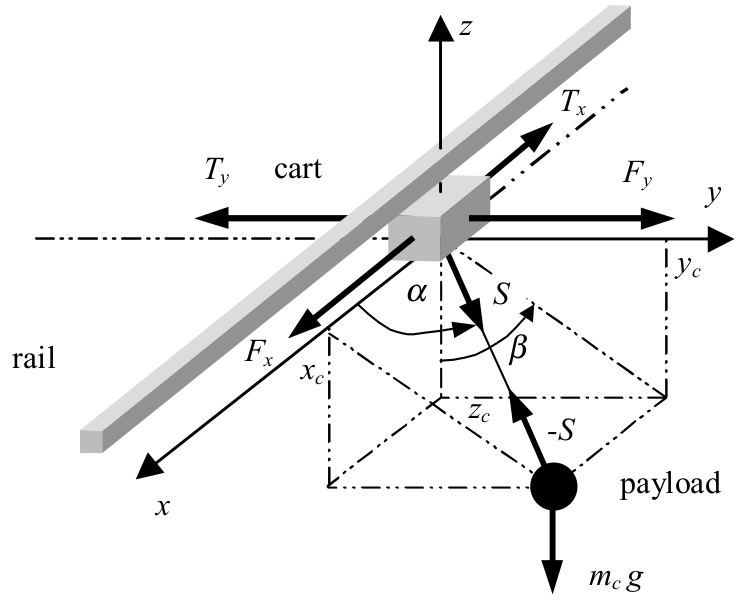
\includegraphics[width=14cm]
    {../res/img/sch-model.png}
  \end{center}
  \caption{Schemat modelu suwnicy}
  \label{sch:model}
\end{figure}

Układ równań stanu dany jest zależnościami \eqref{equ:rstanu},
\eqref{equ:rstanu_n} oraz \eqref{equ:rstanu_v} \cite{agh:crane}.

\begin{equation}
  \begin{cases}
    \dot{x_1}=x_2\\
    \dot{x_2}=N_1+\mu_1\cos{x_5}N_3\\
    \dot{x_3}=x_4\\
    \dot{x_4}=N_2+\mu_2\sin{x_5}\sin{x_7}N_3\\
    \dot{x_5}=x_6\\
    \dot{x_6}=\left(\sin{x_5}N_1-\cos{x_5}\sin{x_7}N_2+(\mu_1-\mu_2\sin^2{x_7})\cos{x_5}\sin{x_5}N_3+V_5\right)\frac{1}{x_9}\\
    \dot{x_7}=x_8\\
    \dot{x_8}=-\left(\cos{x_7}N_2+\mu_2\sin{x_5}\cos{x_7}\sin{x_7}N_3+V_6\right)\frac{1}{\sin{x_5}x_9}\\
    \dot{x_9}=x_{10}\\
    \dot{x_{10}}=-\cos{x_5}N_1-\sin{x_5}\cos{x_7}N_2-(1+\mu_1\cos^2{x_5}+\mu_2\sin^2{x_5}\sin^2{x_7})N_3+V_7\\
  \end{cases}
  \label{equ:rstanu}
\end{equation}

\begin{equation}
  \begin{cases}
    V_5=\cos{x_5}\sin{x_5}x_8^2x_9-2x_{10}x_6+g\cos{x_5}\cos{x_7}\\
    V_6=2x_8(\cos{x_5}x_6x_9+\sin{x_5}x_{10})+g\sin{x_7}\\
    V_7=\sin^2{x_5}x_8^2x_9+g\sin{x_5}\cos{x_7}+x_6^2x_9\\
  \end{cases}
  \label{equ:rstanu_v}
\end{equation}

\begin{equation}
  \begin{cases}
    N_1=u_1-k_1x_2\\
    N_2=u_2-k_2x_4\\
    N_3=u_3+k_3x_{10}\\
  \end{cases}
  \label{equ:rstanu_n}
\end{equation}

\vspace{0.2cm}
\noindent
gdzie zmienne stanu równania to:

\vspace{0.5cm}
\begin{tabular}{R{0.5cm}clcl}
  $x_1$ & = & $x_w$ & -- & Pozycja wózka w osi $x$\\
  $x_2$ & = & $\dot{x}_w$ & -- & Prędkość wózka w osi $x$\\
  $x_3$ & = & $y_w$ & -- & Pozycja wózka w osi $y$\\
  $x_4$ & = & $\dot{y}_w$ & -- & Prędkość wózka w osi $y$\\
  $x_5$ & = & $\alpha$ & -- & Pozycja kątowa liny nośnej względem osi $x$\\
  $x_6$ & = & $\dot{\alpha}$ & -- & Prędkość kątowa liny nośnej względem osi $x$\\
  $x_7$ & = & $\beta$ & -- & Pozycja kątowa rzutu liny nośnej na płaszczyznę
  $yz$ względem osi $z$\\
  $x_8$ & = & $\dot{\beta}$ & -- & Prędkość kątowa rzutu liny nośnej na płaszczyznę
  $yz$ względem osi $z$\\
  $x_9$ & = & $R$ & -- & Długość liny nośnej\\
  $x_{10}$ & = & $\dot{R}$ & -- & Prędkość rozwijania liny nośnej\\
\end{tabular}
\vspace{0.5cm}

\vspace{0.2cm}
\noindent
a parametry równania to:

\vspace{0.5cm}
\begin{tabular}{R{0.5cm}cl}
  $\mu_1$ & = & $\frac{m_c}{m_w}$\\
  $\mu_2$ & = & $\frac{m_c}{m_w+m_s}$\\
\end{tabular}
\vspace{0.5cm}

\subsection{Model uproszczony}

Powyższy model sprawiał trudności podczas obliczeń numerycznych, dlatego do
dalszych rozważań przyjęty został uproszczony układ równań stanu, spełniający
\eqref{equ:rstanu_simp}. Takie uproszczenie oznacza tyle, że lina nośna suwnicy
ma stałą długość $1[m]$.

\begin{equation}
  \begin{cases}
    x_9=1\\
    x_{10}=0\\
  \end{cases}
  \label{equ:rstanu_simp}
\end{equation}

\newpage

\section{Algorytm wyznaczania sterowania}



\newpage

\printbibliography

\end{document}